\section{Project Schedule and Resource Allocation} \label{sec:psara}
%Identify the tasks for your project and their schedule. Do so retrospectively, assuming that the project has started in October 16, 2016 as it really happened.
%Allocate the resources (all members of your group) to the various tasks. In defining the allocation, take into account your actual availability for the project.


In this section, we are going to show a general, high-level project schedule and a general overview of the tasks division between the two members of the our team. We think it is more suitable to define more detailed schedules during the development phases of our project, in order to manage the internal organization in a better way, highlighting the difference of each phase.

During the scheduling definition, we decided to be as coherent as possible to the results of the analysis described in the previous sections (Section \ref{sec:functpointappr} and Section \ref{sec:cocomo}) but adapting them to our specific case, that is a team with two members.

The project scheduling consist in deciding how the work in a project will be organized as separate tasks, and when and how these tasks will be executed.
So, we need to estimates the calendar time needed to complete each task, the effort required, who will work on the tasks that have been identified and the resources needed to complete each task.

In order to fully develop our project, we have identified $6$ different tasks:

\begin{itemize}

\item[\textbf{T1}]: feasibility study;

\item[\textbf{T2}]: analysis of requirement and specification;

\item[\textbf{T3}]: design of the system;

\item[\textbf{T4}]: coding and unit testing;

\begin{itemize}

\item[\textbf{T4.1}]: client side;

\item[\textbf{T4.2}]: server side;

\item[\textbf{T4.3}]: database;

\end{itemize}

\item[\textbf{T5}]: integration test and system test;

\item[\textbf{T6}]: deployment;

\end{itemize}

We decided to represent our schedule using a bar chart, since graphical notations are normally used to illustrate the project schedule.
Moreover, we tried to grand an equal workload for each team member, so we have developed the following Gantt diagram, showing the distribution of every task during the months, forecasting a total duration of 14 months (since we want to balance the results obtained by the evaluation with \acs{cocomo} II: our team is composed by $2$ people, instead of the $2.56$ resulting from the estimation).

\begin{figure}[htbp]
\centering
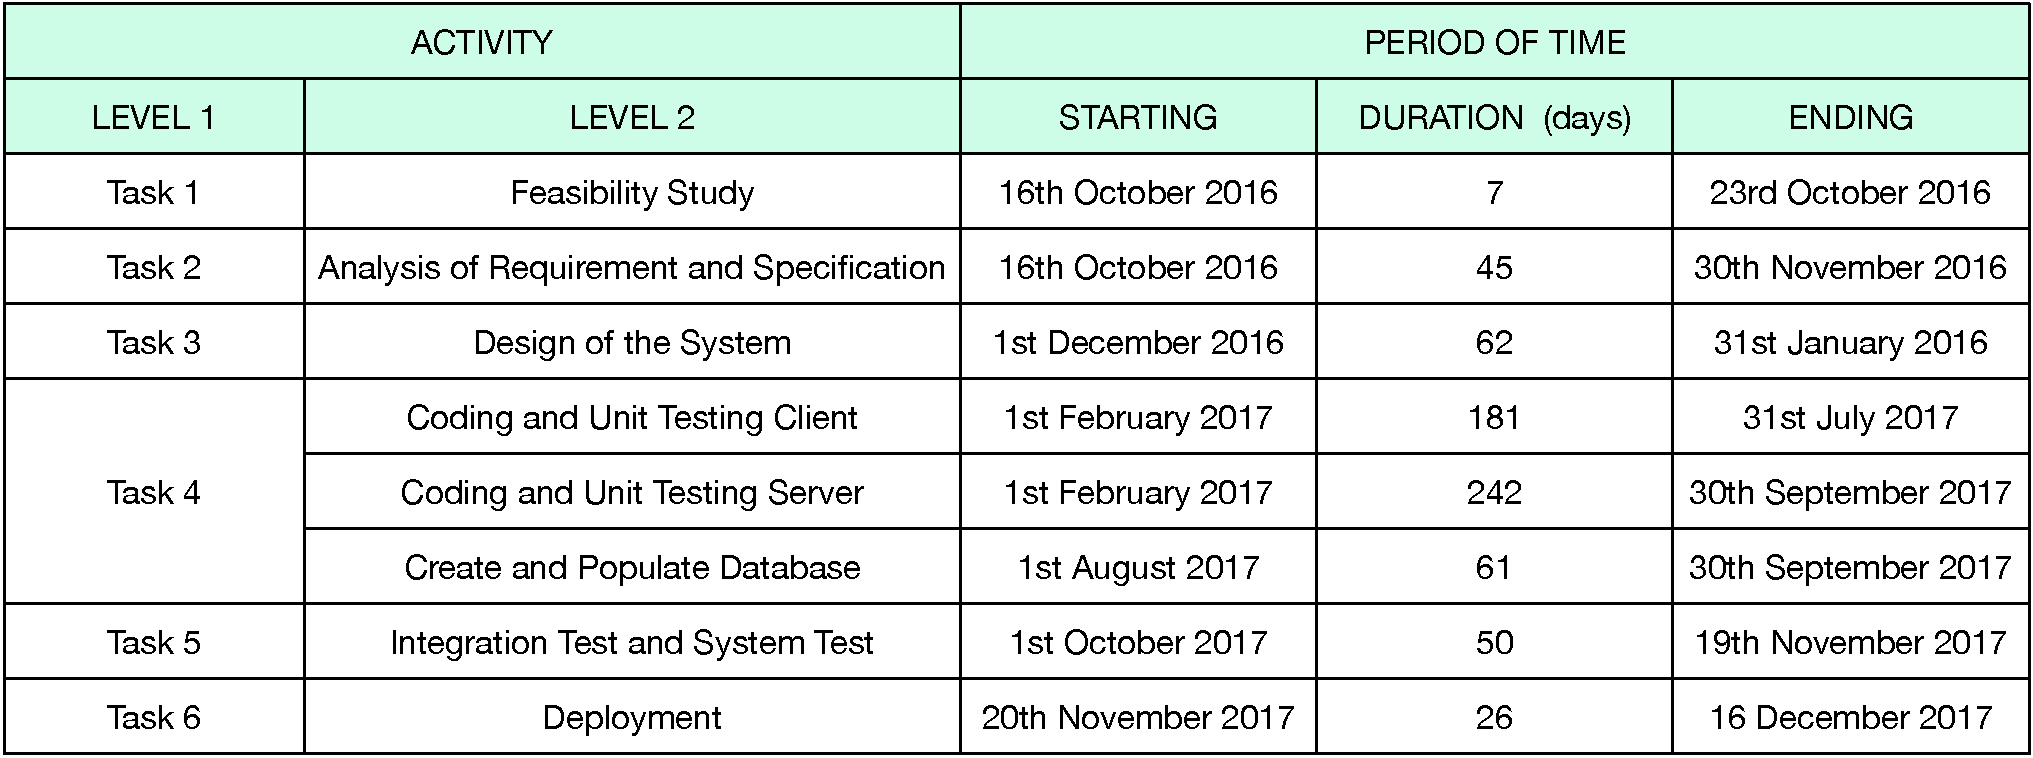
\includegraphics[width=\textwidth]{Images/scheduling}
\caption{Project Scheduling}
\label{fig:sched}
\end{figure}

\begin{figure}[htbp]
\centering
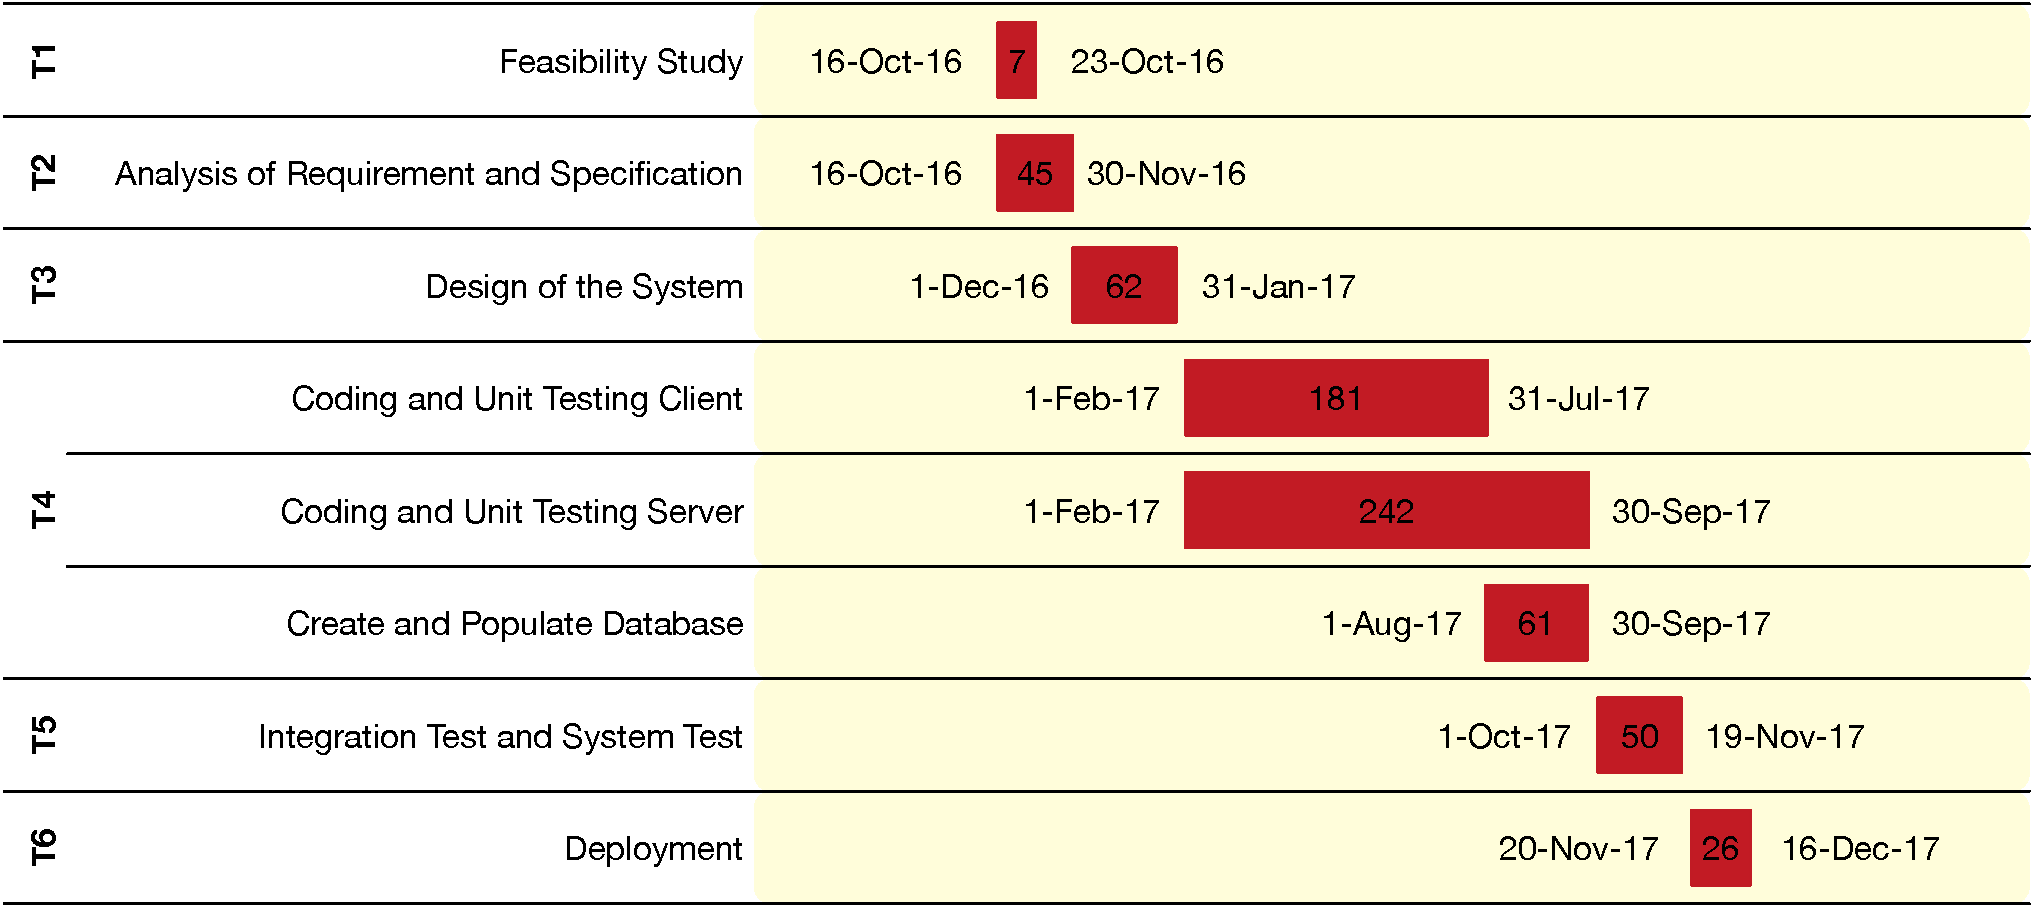
\includegraphics[width=\textwidth]{Images/scheduling_bar_chart}
\caption{Graphical Represenattion of Project Scheduling}
\label{fig:chart_sched}
\end{figure}

\clearpage

In Figure \ref{fig:alloc}, we are showing the reader how the staff will be allocated in order to accomplish each task.

\begin{figure}[htbp]
\centering
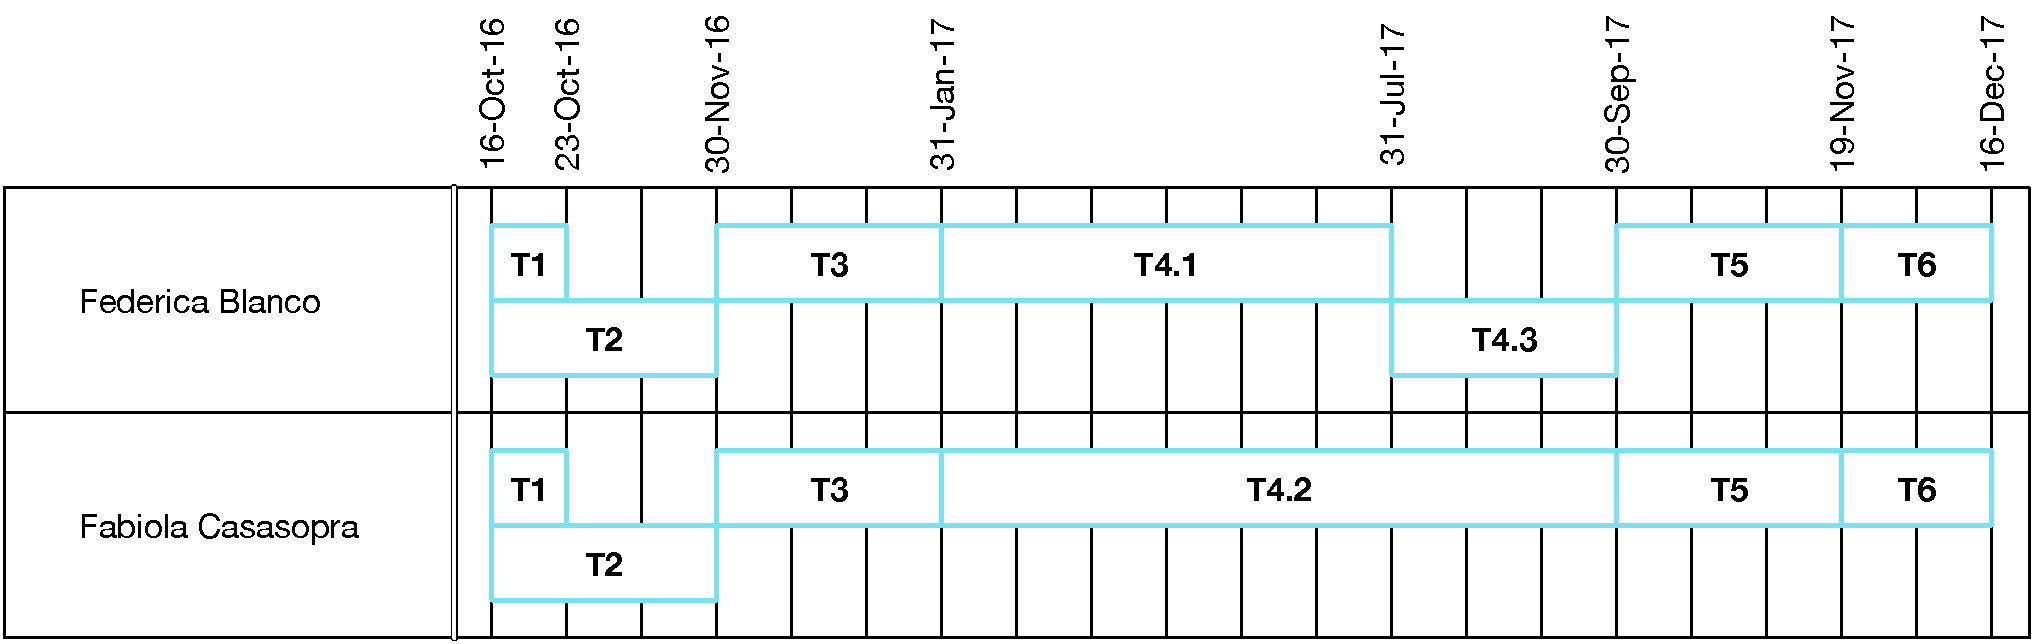
\includegraphics[width=\textwidth]{Images/staff_allocation}
\caption{Staff Allocation}
\label{fig:alloc}
\end{figure}



